\subsection{Electrical Results}

\begin{frame}{Different cable lengths}
    \begin{figure}
        \includesvg[width=0.8\textwidth]{../../documentation/graphics/different_cable_lengths_with_dso_tdc.svg}
    \end{figure}
    \iconelectrical
\end{frame}

\begin{frame}{Different cable lengths: Results}
    \begin{table}
        \mytable
        {|l|l|l|l|}
        {\textbf{Length} & \textbf{Mean} & \textbf{Standard deviation} & \textbf{$\Delta$ at 0~m}}
        {\length & \mean & \stddev & \diff}
        {../../documentation/tables/different_cable_lengths_with_dso_tdc.csv}
    \end{table}
    \iconelectrical
\end{frame}

\begin{frame}{Different cable lengths: Calculated backwards}
    \begin{table}
        \mytable
        {|l|l|}
        {\textbf{Length} & \textbf{TDC recalculated with 0.9~c}}
        {\length & \tdcgemtheoriemc}
        {../../documentation/tables/different_cable_lengths_with_dso_theorie09_vs_tdc_m.csv}
    \end{table}
    \iconelectrical
\end{frame}

\subsection{Optical Results}

\begin{frame}{Signal Path Transmitter}
    \begin{figure}
        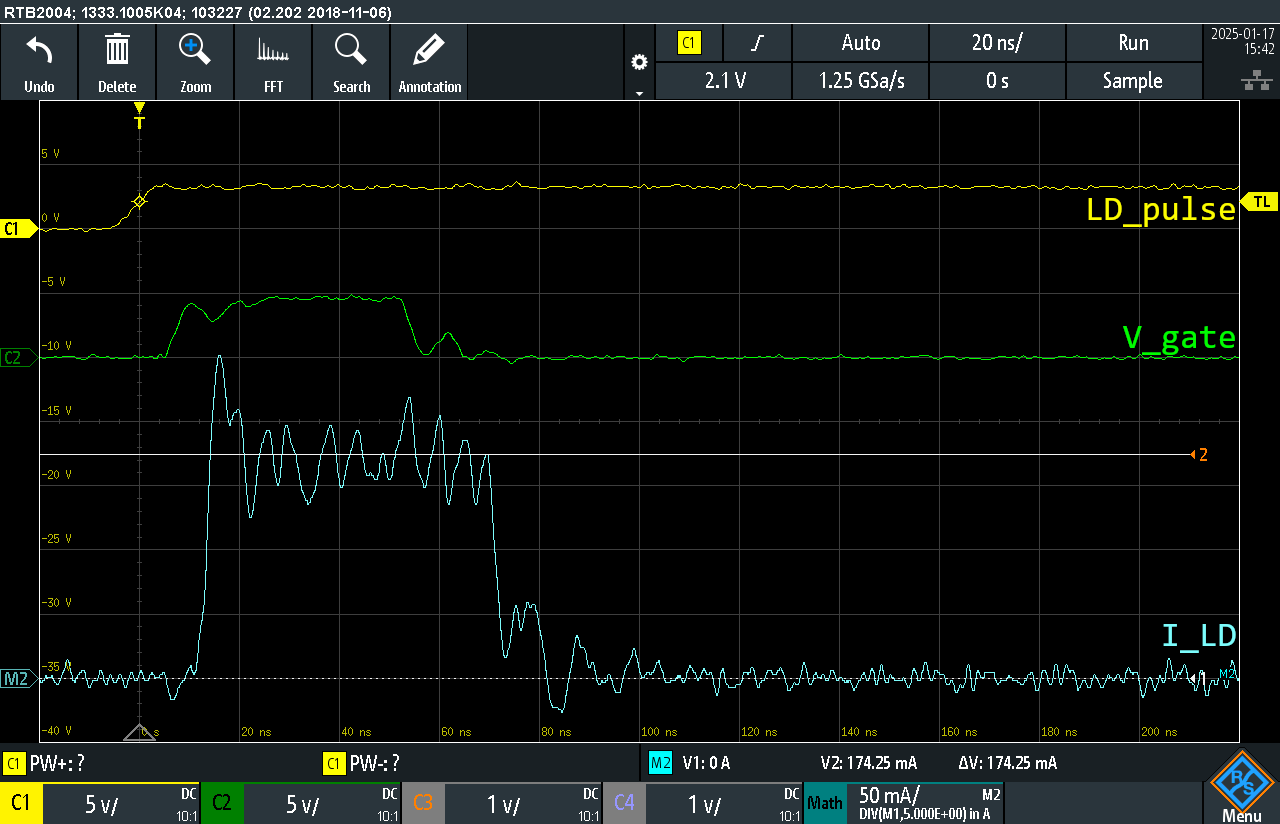
\includegraphics[width=0.7\textwidth]{../../documentation/graphics/signalpfad_sender_ld_strom.png}
    \end{figure}
    \iconoptical
\end{frame}

\begin{frame}{ToF measurements via mirror}
    \begin{figure}
        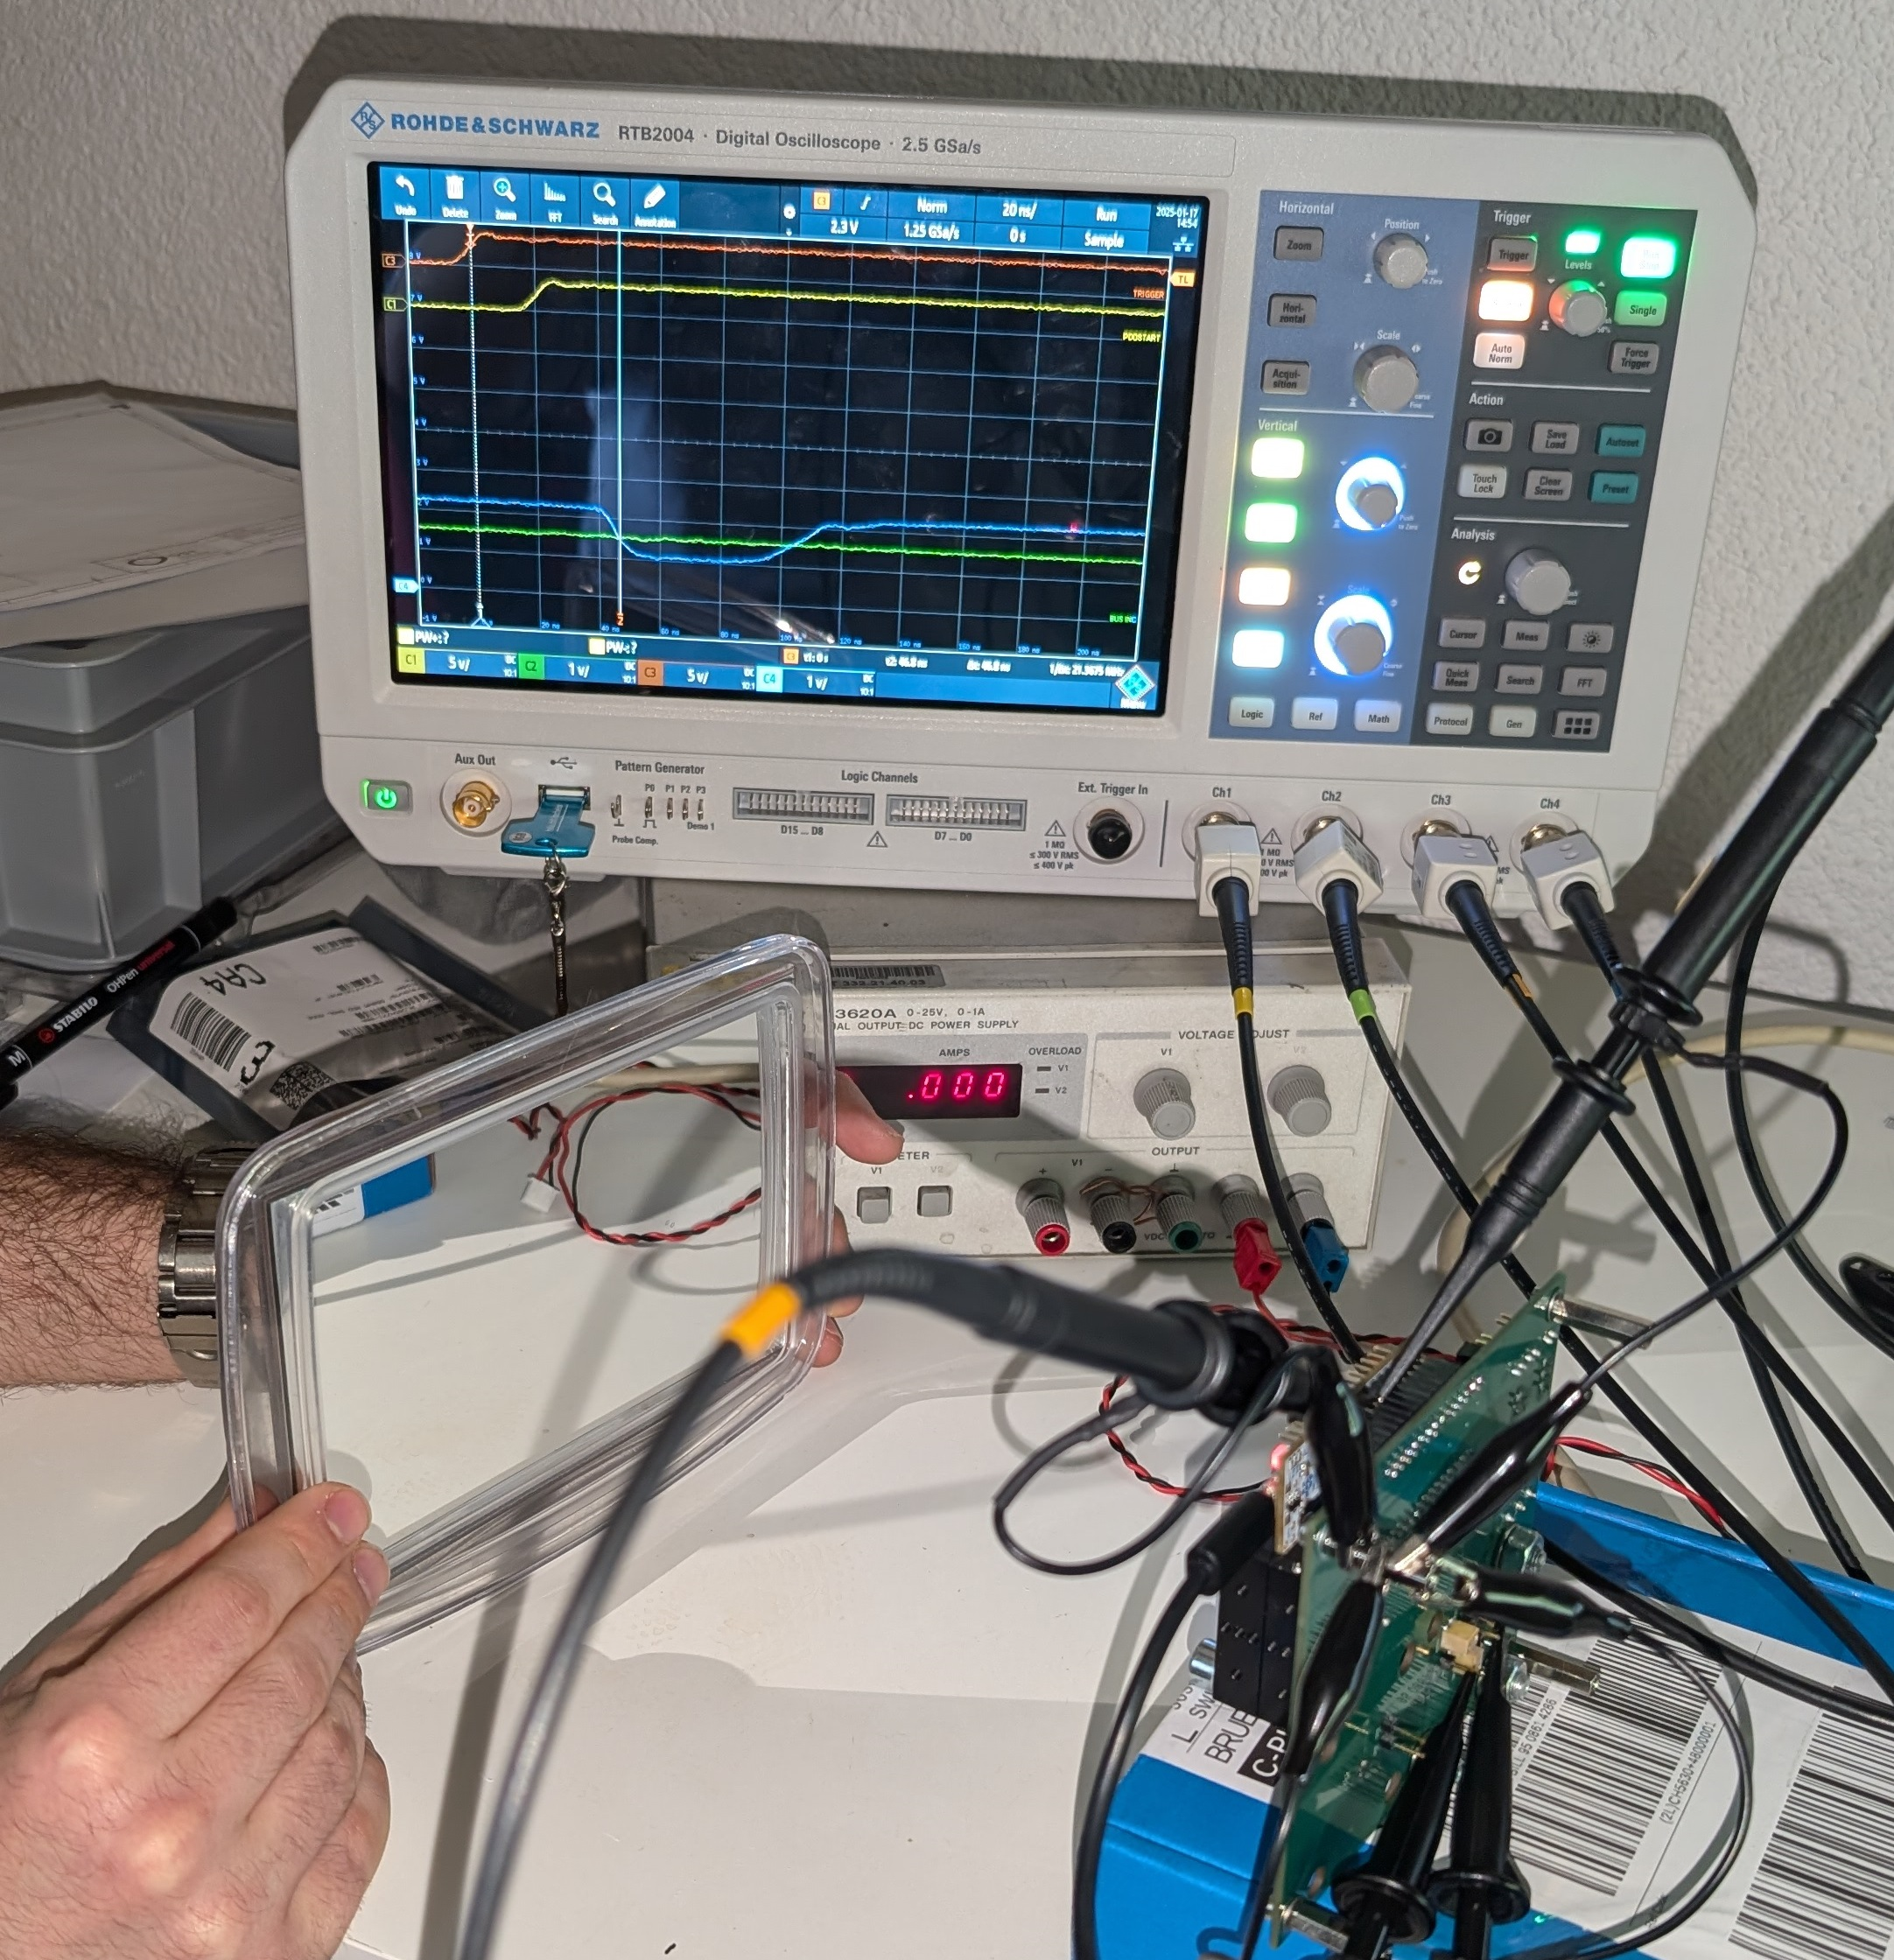
\includegraphics[width=0.45\textwidth]{../../documentation/graphics/spiegel_setup.jpg}
    \end{figure}
    \iconoptical
\end{frame}

\begin{frame}{ToF measurements via mirror: DSO}
    \begin{figure}
        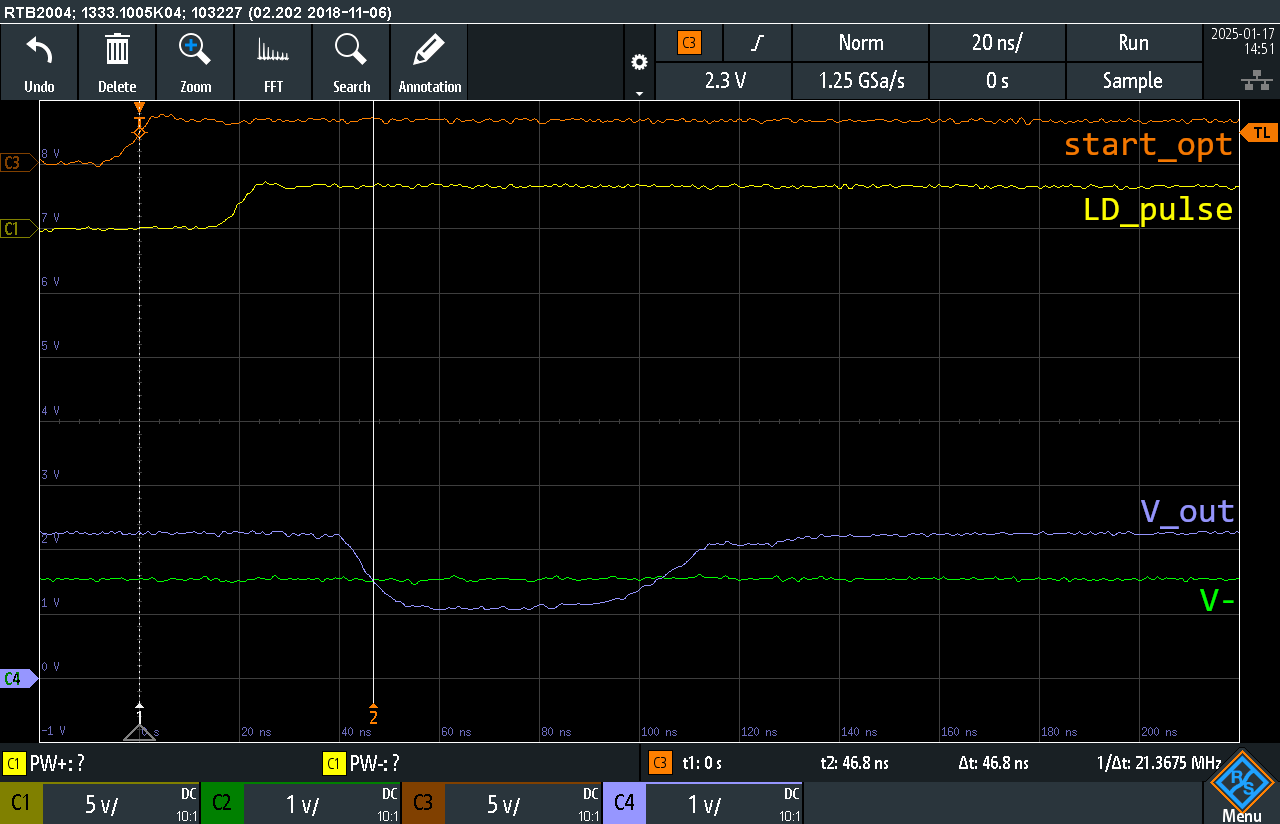
\includegraphics[width=0.7\textwidth]{../../documentation/graphics/spiegel_12cm_dso_ok.png}
    \end{figure}
    \iconoptical
\end{frame}

\begin{frame}{ToF measurements via mirror: Results}
    \begin{figure}
        \includesvg[width=0.8\textwidth]{../../documentation/graphics/spiegel_unterschiedliche_distanzen.svg}
    \end{figure}
    \iconoptical
\end{frame}

\begin{frame}{ToF measurements via mirror: analysis}
    \begin{table}
        \mytable
        {|l|l|l|}
        {\textbf{Distance to mirror} & \textbf{Mean value} & \textbf{Standard deviation}}
        {\distance & \mean & \stddev}
        {../../documentation/tables/spiegel_unterschiedliche_distanzen.csv}
    \end{table}

    \onslide<2->{
        \begin{equation*}
            \begin{split}
                \Delta ToF_{meas} & \approx 0.6~ns                                                  \\
                \Delta ToF_{calc} & = \frac{\Delta L}{c} = \frac{10~cm}{3 \cdot 10^8~m/s} = 0.33~ns
            \end{split}
        \end{equation*}
    }
    \iconoptical
\end{frame}

\begin{frame}{ToF measurements via mirror: drift}
    \begin{figure}
        \includesvg[width=0.8\textwidth]{../../documentation/graphics/spiegel_unterschiedliche_distanzen_linear.svg}
    \end{figure}
    \iconoptical
\end{frame}

\begin{frame}{ToF measurements via mirror: $>$30 cm}
    \begin{figure}
        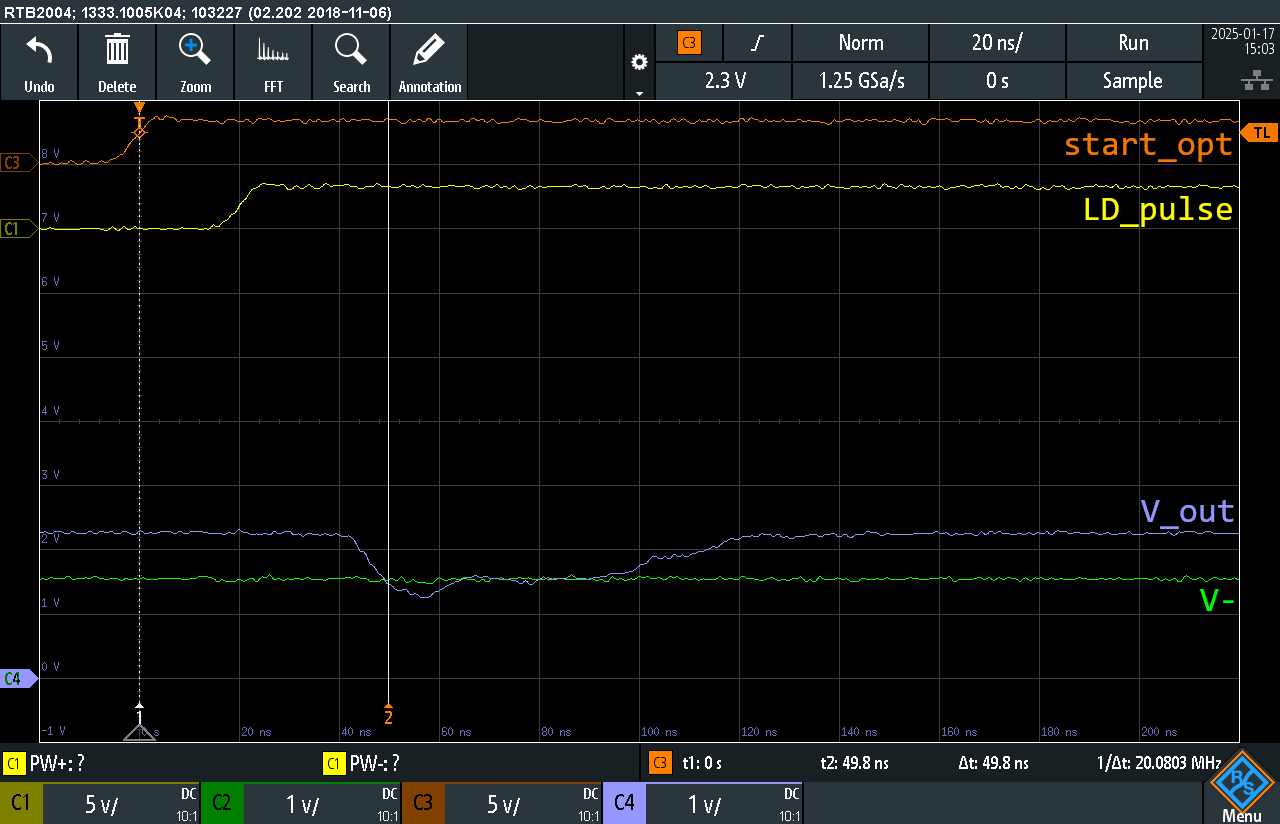
\includegraphics[width=0.7\textwidth]{../../documentation/graphics/spiegel_30cm_dso_nok.png}
    \end{figure}
    \iconoptical
\end{frame}

\begin{frame}{ToF measurements via wall}
    \begin{itemize}
        \item Unfortunately, optics not yet designed for this
    \end{itemize}
    \iconoptical
\end{frame}
